\chapter{The Diffusion of Spices}
\label{ch:diffusion}

% Empirical Chapters
% Discuss and present your findings in a factual way.
% What are the results of your investigations?
% How do the findings relate to previous studies?
% Was there anything surprising or that didn’t work out as planned?
% Are there any themes or categories that emerge from the data?



\lettrine[lines=\iniciale]{\textcolor{\accentcolor}{I}}{n} this chapter, I will present the findings on the diffusion of spices, through the investigation of spice names and their spread on spatial and temporal dimensions. In order to present these results in a convenient, reader friendly way, I will use geospatial mapping. The plots seen in this chapter are made by using the etymological data on spice terminology, collected and introduced in \cref{ch:data}.



Fig X shows the spatial trajectory of all English words included in the set, and we can observe a few trends off glance. First of all, there is a   

PEPPER


% --------------------------------------------

\section{The Case of Cinnamon}
\label{ch:cinnamon}

\section{One}

% Empirical Chapters
% Discuss and present your findings in a factual way.
% What are the results of your investigations?
% How do the findings relate to previous studies?
% Was there anything surprising or that didn’t work out as planned?
% Are there any themes or categories that emerge from the data?

This chapter aims to give an overview on the terminology used by various languages when referring to cinnamon. These words are connected to the spread of material culture, and a (not-so) specific plant product used and coveted for its aroma, used as spice and medicine. Known by humans for millennia, cinnamon is now present essentially on a global scale, and by exploring its names in multiple languages, we can reconstruct its linguistic genealogy. These results also tell a story; they tell us an account on the linguistic history of \emph{cinnamonic} words, their origins, diffusion, and ultimately, the story of cinnamon. We can infer information on the trade routes and the peoples who transmitted it, and identify the cultures that used and diffused knowledge on it. 

\begin{figure}[ht!]
    \centering
    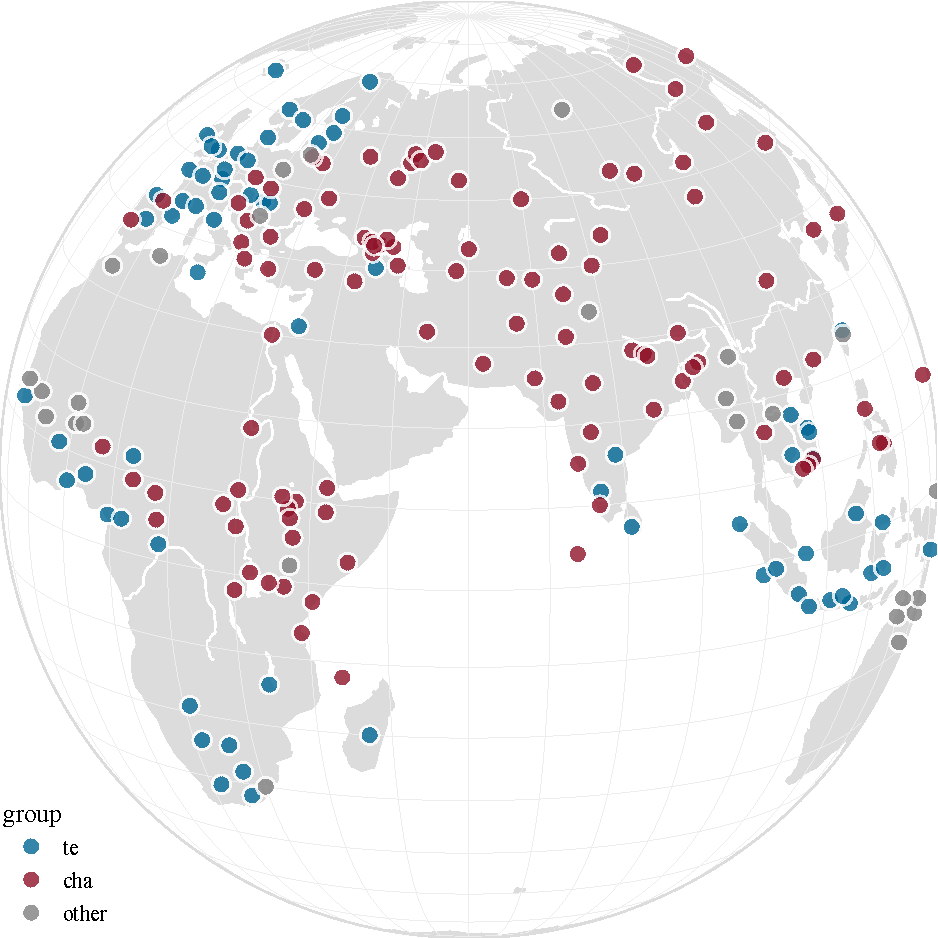
\includegraphics[width=\linewidth]{imgs/plots/distribution_tea.pdf}
    \caption{Distribution of words for tea from Sinitic \textit{cha} and Minnan \textit{te}, based on the data around the globe.}
    \label{fig:distribution_tea}
\end{figure}

To those of us who interested in the spread of words, especially \glspl{wanderwort} and their underlying cultural, historical, and geo-political significance, the map of tea might come to mind. This is a map that shows the journey of words for tea (either from Sinitic \textit{cha} or Minnan \textit{te}), and their distribution in a sample of the world's languages. The point of this map is that it clearly shows if the name for tea arrived by overland trade or via a sea route. This peculiar phenomenon is a feature on its own (138A) in \gls{WALS}, and have been described in a chapter by \textcite{dahl_tea_2013}.\footnote{The accompanying map is available online at \url{https://wals.info/feature/138A\#2/25.5/143.6}} Discussions and maps of the land vs. sea distribution of tea terminology have since made it into popular science magazines and articles, made rounds on Twitter, and hence relatively well known.\footnote{See for example \textcite{sonnad_tea_2018} in Quartz: \url{https://qz.com/1176962/map-how-the-word-tea-spread-over-land-and-sea-to-conquer-the-world/} or \textcite{netchev_movement_2022} in the World History Encyclopaedia: \url{https://www.worldhistory.org/image/14112/movement-of-tea--cha-around-the-globe/}} On a more scientific note, the distribution of tea words are discussed in detail by \parencite[261-270]{mair_true_2009} in an appendix titled \textit{A Genealogy of Words for Tea}, with including a discussion on historical phonology.

Cinnamon as a spice is relatively well known around the world, and the history of its diffusion goes back to thousands of years, with words attested as early as the Bible itself, as it was discussed in \cref{sec:cinnamon}. This is in contrast with the story of tea, in the sense that the international spread of tea is a relatively recent process in the economic history of plant products and colonial powers, and so we have a much clearer picture on the exact ways it was transmitted. Although tea-drinking in its homeland was practiced from time immemorial, and trade allowed it to spread regionally on networks, such as the Tea Horse Road, its present global domination is a result of \nth{17}-century European fascination and large scale shipping. While the tea map illustrates the long haul trade connections of the time, such as those between Europe and the Far East, the map of cinnamon shows traces of an older, more gradual spread that happened in stages, outlining a more geographically contiguous development, and incremental trade networks. The propagation of cinnamonic \glspl{wanderwort} mirrors the historical processes, and just as the story of cinnamon, the words' origins are sometimes obscured by the sheer time-depth that is covered.

\section{Methods and Data}

Informative geospatial visualizations such as \cref{fig:distribution_tea} above are a powerful tool in conveying the information about spread and distribution of words, and they can also help us to notice patterns and connections faster and easier than studying long tables of words, especially when the distributions are more complex than the somewhat neat duality of tea. In this case study, I will attempt a classification for the words for cinnamon by looking at clusters and categorizing them according to their source, to see what the distribution of names today can tell us about the spread and history of cinnamon.

Because words for cinnamon or other spices are not included as features in balanced typological datasets, such as \gls{WALS} (tea is an exceptional feature in this database), I have attempted a manual collection of words for cinnamon based on dictionary entries. As a starting point, I have crawled data from the \gls{wiktionary} (\url{https://en.wiktionary.org}), which is the closest resource we currently have to an open- and crowd-sourced multilingual dictionary. Similarly to the Wikipedia, the Wiktionary is edited and reviewed by the community, which has both advantages and disadvantages. On one hand, information on the Wiktionary is free, broad in scope, it usually represents the public consensus, and often well cited. On the other hand, it is not always complete, the available languages do not represent a balanced sample from a typological point of view, and the information can sometimes be ill-informed or deprecated. In any case it is a rich resource to start with. 

For cinnamon, first I scraped the translations for the word \textit{cinnamon} in the sense `spice' \parencite{wiktionary_cinnamon_nodate}, and cleaned the data using regular expressions. After this, I have performed a round of manual checking where I fixed obvious mistakes in word forms and transliterations by consulting other dictionaries and reference works, in the languages and scripts I felt competent to do so. I proceeded to add a few missing translations with the help of other lexicographical resources and the Google Neural Machine Translation engine's Python API \parencite{wu_googles_2016}.\footnote{\url{https://pypi.org/project/googletrans/}} Then, I analyzed each word in terms of etymological origin, and assigned them to categories. For example, words derived from Greek \textit{kinnámōmon}, such as Lithuanian \textit{cinamonas} or English \textit{cinnamon} constitute one category, and words derived from Persian \textit{dârčin}, such as Turkish \textit{tarçın} or Hindi \textit{dālcīnī}, make up another. I continued this categorization for all instances, and created a new category for every group that has at least three attested members. Instances that do not belong to any group or undetermined were assigned to ``other''. Finally, I merged this dataset with language data obtained from the databases of both \gls{WALS} \parencite{dryer_wals_2013} and \gls{glottolog} \parencite{hammarstrom_glottolog_2022} to prepare for geospatial plotting. The datasets were handled using the \texttt{pandas} library in Python, and the visualizations were created using the \texttt{plotly} Python library \parencites{pandas, plotly}.

\section{Results and Discussion}

\Cref{fig:cinnamon_distribution} shows the results of the analysis above, on a geographical scatter plot. As it can be seen, there are six groups in total: canela, kinnamon, korica, qirfa, darchin, and gui, with a seventh one --- other --- containing those that do not belong to any of these. It is also noticeable that the groups that were manually identified form geographical clusters, for example, the gui group appears in East Asia, while the canela group is mainly found in Europe. Lastly, I would like to draw attention that the ``other'' group has a high number of members in regions where cinnamon (or cassia) is native. The canela group represent words that derived from Latin, the kinnamon group contains words going back to Greek, and the korica group represent mostly Slavic languages. Qirfa words are derived from Arabic, darchin gathers terms from the Persianate world, and gui embraces some terms from the Sinosphere. Let us now look at these categories one by one.

\begin{figure}[!ht]
    \centering
    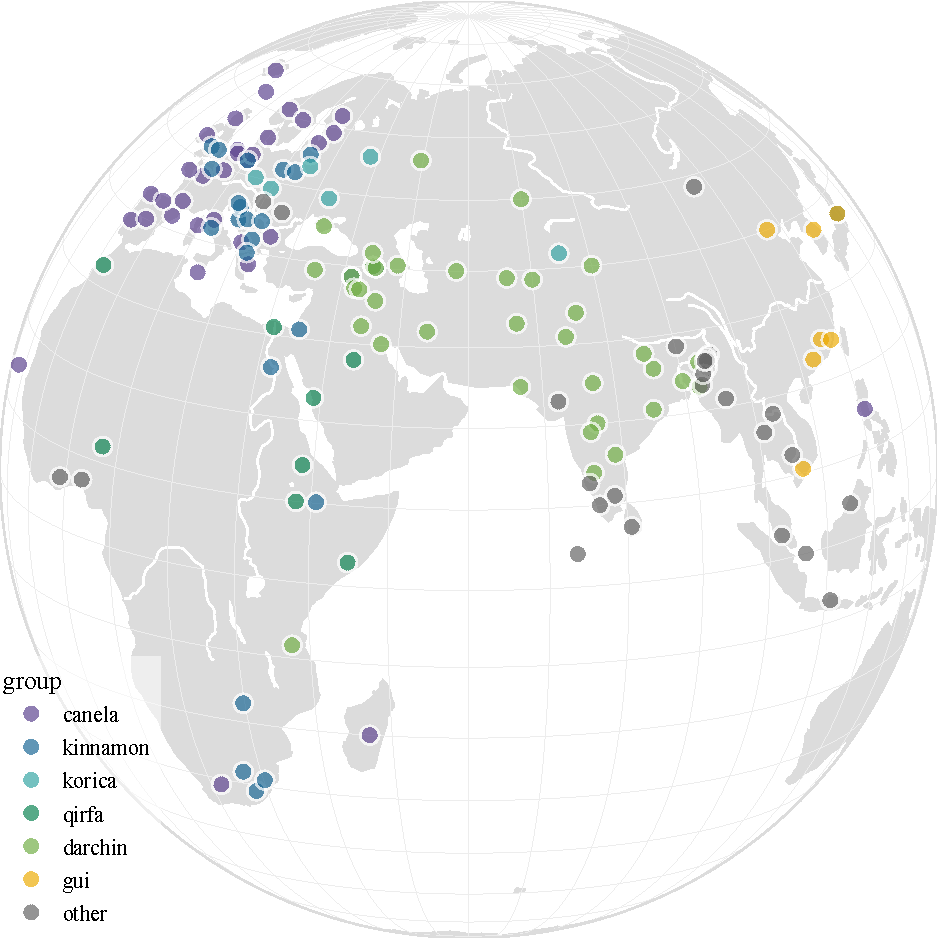
\includegraphics[width=\linewidth]{imgs/plots/distribution_cinnamon.pdf}
    \caption{The distribution of \textit{cinnamonic} words in a few languages around the globe.}
    \label{fig:cinnamon_distribution}
\end{figure}

\begin{note}
For a full, interactive and explorable version of the plot, please visit the following link: \url{http://htmlpreview.github.io/?https://github.com/partigabor/phd-test/blob/main/cinnamon.html}.\footnote{For an annotated version, please visit \url{http://htmlpreview.github.io/?https://github.com/partigabor/phd-test/blob/main/cinnamon_annotated.html}} The interactive plot can be rotated, zoomed in and out, and the groups of data points can be isolated with a double-click on the group name/icon. Hovering over a data point will bring forward further information on the term, its transliteration, associated language and language family.
\end{note}

\subsection{The canela group}

Words belonging to this group are cognates of Spanish \textit{canela} and its variants in Romance languages, which have been formed with the diminutive of Latin \textit{canna} `reed, cane'. It is named so after the curled shape of the cinnamon sticks resembling a little, hollow reed-pipe \entry{OED}{cannel}. Latin \textit{canna} itself is a loanword from Greek \gr{κᾰ́ννᾱ}
\textit{kánna} `reed, pole', which is probably a borrowing from a Semitic language (cf. Arabic \ar{قناة}
\textit{qan\={a}h} `hollow spear, cane; conduit, canal', Hebrew \he{קָנֶה}
\textit{qāneh} `stalk, reed, cane', Aramaic \sy{ܩܢܝܐ} 
\textit{qanyā} `id.'\footnote{\url{https://cal.huc.edu/oneentry.php?lemma=qnh+N&cits=all}}) \entry{OED}{cane}. According to \textcite[636]{beekes_etymological_2010} the Greek word is from ``Babylonian-Assyrian'' (Akkadian) \cu{\GA\NU\UU\UM} \textit{qanû} `reed', which may come from ``Sumerian-Akkadian'' (Sumerian) \cu{\GI} \textit{gin} `id.' \pvolcite[cf.]{13}[85]{roth_assyrian_2004}, and proceeds to give Ugaritic \textit{qn} and Punic \textit{qn'} as further Semitic attestations.

The distribution of this group is overwhelming in Europe, which seems to echo the strong influence of Latin vocabulary, especially in the developing Romance languages. One example would be Old French \textit{canele} (modern \textit{cannelle}), which was formed within French from \textit{canne} `cane', and first attested in the first half of the \nth{12} century from an epic poem describing a fictional expedition of Charlemagne to Jerusalem\footnote{\textit{Le Pèlerinage de Charlemagne [The Pilgrimage of Charlemagne]}, or \textit{Voyage de Charlemagne à Jérusalem et à Constantinople [Charlemagne's Voyage to Jerusalem and Constantinople]}, (c. 1140).}, and the local vendors selling cinnamon, pepper, and ``other fine spices'' \entry{TLFi}{cannelle}\footnote{\url{https://www.cnrtl.fr/definition/cannelle}}. The \gls{TLFi} explains that this word exists in most romance languages and it is impossible to determine its progress, and also notes that the medieval Latin is not attested in the `cinnamon' sense. Either French or Italian was the usual donor for other European languages, take for example Dutch \textit{kaneel}, or Finnish \textit{kaneli} through Swedish \textit{kanel}. Spanish \textit{canela} is attested around 1250, from ``Italian'' (Medieval Latin) \textit{cannella} \parencites[125]{corominas_breve_1987}[98]{gomez_de_silva_elseviers_1985}. Due to later colonization by European powers, many of these terms spread elsewhere, e.g.: Tagalog \textit{kanela} from Spanish, or Haitian Creole \textit{kannèl}.

\textit{\obs Cannel}, also earlier as \textit{canel} had entered English usage in the \nth{13} century from French, but is now obsolete. It existed in Early Modern English up until the \nth{18} century, and was gradually replaced by \textit{cinnamon} (also arriving through French), which was first attested in the first half of the \nth{15} century (see Etymology \ref{ety:cinnamon}). Neo Latin \textit{canella} also appeared for a brief time, but its meaning as `cinnamon' waned, and now it is used in botany to refer to a plant genus.

In many other languages of Europe the opposite happened, and an existing word from Greek was replaced by the Latin term. Even Modern Greek uses \textit{kanéla}, re(?)-borrowed from Italian \textit{cannella}, instead of the Ancient Greek \textit{kinnámōmon}. 

\subsection{The kinnamon group}

This group centers around Ancient Greek \textit{kinnámōmon}, most possibly a loanword from a Semitic language as I discussed in \cref{sec:cinnamon_names_en}. \textit{Kinnámōmon} is the source of words for cinnamon in many European languages (e.g.: German \textit{Zimt}, Lithuanian \textit{cinamonas}, and English \textit{cinnamon}), prominently in Central Europe and the Middle East. In most cases, these words represent an area where words derived from Latin cannella (or one of its descendants) did not replace the earlier word derived of \textit{kinnámōmon}. This group also contains South Slavic languages in the Balkan linguistic area (e.g. Slovenian \textit{cimet}, Serbian \cy{цимет} \textit{cimet}) where it arrived via the earlier German term \textit{Zimmet} (now \textit{Zimt}), and therefore it diverges from West and East Slavic branches for this lexical item. It reached Southeast Europe in the \nth{16} century \parencite[s.v. cimet]{snoj_slovenski_1997}\footnote{Fran --- \url{https://fran.si/193/marko-snoj-slovenski-etimoloski-slovar/4285437/cimet?View=1\&Query=cimet}}, from which we can assume that cinnamon started to arrived here from the West during this turbulent time in the Balkans, in the middle of the Ottoman Empire's European expansion.

\subsection{The korica group}

The korica group contains languages that use words derived from the inherited Slavic lexicon, in this case the East and West Slavic branches. Proto-Slavic \textit{*korica} `bark' is a derivative of \textit{*korà} `bark'\footnote{\gls{PIE} \textit{*(s)kor-} `to cut' ??}, the suffix \textit{-ica} is diminutive. Old Church Slavic \textit{koricę} meant `cinnamon', and further cognates are Russian \textit{koríca} `id.', Ukrainian \cy{кори́ця} \textit{korýcja} `id.' (East Slavic), Czech \textit{skořice} `id.' (West Slavic). In other cases, words derived from \textit{*korica} can mean `bark, crust' (e.g. Serb-Croatian) or `cover (of a book), binding' (e.g. Bulgarian) \parencite[235]{derksen_etymological_2008}. Due to the influence of Russian during Soviet times, some Central Asian Turkic languages ended up with a foreign words in their vocabularies, e.g. Kirghiz \cy{корица} \textit{korica} ??.

\subsection{The qirfa group}

The qirfa group contains languages from Africa and the Middle East, whose words for cinnamon were borrowed from Arabic \textit{qirfa}, for example Hausa \textit{kirfa} \parencite[114]{newman_hausa-english_2007} and Amharic \am{ቀረፋ} \textit{qäräfa} \parencite[74]{leslau_concise_1996}.

\subsection{The darchin group}

Names for cinnamon in this category originate from Persian, as it was explained in \cref{sec:cinnamon_names_ar}. According to the data this cluster has the largest geographical extent, and by number of instances constitutes the largest group, almost head to head with the group of canela. Darchin represents the earliest stage of cinnamon's westward spread from South, Southeast, or East Asia, depending which cinnamon or cassia we think became the first cinnamon of commerce. Consulting the plot we can witness the huge influence Persian had in this step of transmission to the Middle East and Central Asia. We can also see that central and north Indian languages use a loanword from Persian, which can be explained by the Persianate\footnote{For a discussion on this term, see \textcite{green_persianate_2019}.} societies that resulted from the Islamic conquest of India, starting from the \nth{13} century. The first sultan to ravage the land, Mahmud of Ghazni was a Persianized \textit{mamluk} Turk, who laid the foundations with his raids in the \nth{11} century for a series of Muslim dynasties on the Indian subcontinent, culminating in the Mughal Empire (1526–1857) and what we define today as Indo-Persian culture \parencite[33]{eaton_india_2019}.

\subsection{The gui group}

The gui group contains terms from the Sinosphere, words that borrowed the Sinogram \zh{桂} \textit{gui} (see \cref{sec:cinnamon_names_zh}), such as Japanese \jp{桂} \textit{kei} `cinnamon or cassia tree', synonym with \jp{肉桂 (肉桂)} \textit{nikkei}, Korean \ko{계} \textit{gye} as \ko{계피 (桂皮)} \textit{gyepi} and \ko{육계 (肉桂)} and the Sino-Vietnamese \vi{quế}. This shows that the the Chinese transmitted their cassia to their immediate neighbors East and Southwest, together with the word and character for it. However, there is little evidence for trade in cinnamon between China and Southeast Asia in early history, \textcite{wang_nanhai_1958} does not give any information on it in his \citetitle*{wang_nanhai_1958}. \autocite{wang_nanhai_1958} This makes sense if we remember that all regions active in the South China Sea maritime trade --- from Guangdong to Sumatra to Lanka --- had their own source of cinnamon, and traders would only transport it westwards.


\subsection{Others}

We can see that the category of ``other'' is prevalent in areas where cinnamon of various kinds is native and therefore these languages often have native words to refer to it. Many words from these group are derived from the meaning of `tree bark, skin, peel' Malay/Indonesian \textit{kulit kayu manis} [bark-wood-sweet] `sweet wood bark', where \textit{kulit} `skin, bark' is often omitted, or Dhivehi \textit{fonithoshi} [sweet-bark]. 



Hungarian \textit{fahéj} [tree-bark] is made by compounding and was attested in ca. 1395 \parencite[s.v. fahéj]{zaicz_etimologiai_2006},

Romanian \textit{scorțișoară}\footnote{Diminutive of \textit{scoarță} `bark', from Latin \textit{scortum} `hide, skin', PIE *(s)ker- `to cut'.}, is perhaps modeled after Slavic \textit{*korica}.

scortea,

scortum

*(s)ker- (“to cut”)



\section{Two}

So what does this tell us exactly? It shows that in East Asia Chinese, especially the Chinese writing had influence over its neighbors...?






\section{Conclusion}


\section{Limitations}

